% Test-kommentar
\documentclass[openany,12pt,a4page]{memoir}
%
% Packages
%
\usepackage[utf8]{inputenc}
\usepackage[T1]{fontenc}
\usepackage[danish]{babel}


% \usepackage{fouriernc}               % 
% \usepackage{fourier}                 % 
% \usepackage{lmodern}                 % Latin modern
\usepackage{cmbright}                % Computer modern bright
% \usepackage{gfsartemisia-euler}      % GFS Artemisia with Euler math
% \usepackage{mathdesign}              % Math design
% \usepackage{tgschola}                % 
% \usepackage{times}                   % Times
% \usepackage{kpfonts}                 % KP Serif
% \usepackage{DejaVuSerif}             % Deja Vu Serif
% \usepackage[sc]{mathpazo}            % Palatino
% \linespread{1.05}

\usepackage{courier}
\usepackage{icomma}
\usepackage{amsmath,amsfonts,amssymb}
\usepackage{graphicx}
\usepackage{gensymb}
\usepackage{xcolor}
\usepackage{pdfpages}
\usepackage{eurosym}
\usepackage{bbding}
\usepackage{longtable}

%\usepackage{wrapfig}
\usepackage{subfig}
\usepackage[per-mode=fraction,unit-color = black]{siunitx}
\sisetup{output-decimal-marker = {,}}
\usepackage[section]{placeins}
%\usepackage{siunitx}
\usepackage{tikz}
\usepackage{tikz-uml}
\usetikzlibrary{shapes}
\usepackage{pgfplots}
\pgfplotsset{compat=newest}
\pgfplotsset{
  every linear axis/.append style={
    legend pos=outer north east,
    % axis x line=middle, 
    % axis y line=middle,
  },
  every semilogy axis/.append style={
    legend pos=outer north east,
    % axis x line=middle, 
    % axis y line=middle,
  },
  every semilogx axis/.append style={
    legend pos=outer north east,
    % axis x line=middle, 
    % axis y line=middle,
  },
  every loglog axis/.append style={
    legend pos=outer north east,
    % axis x line=middle, 
    % axis y line=middle,
  },
  every axis plot/.append style = {
    thick,
  },
}
\usepackage{listings}
\lstset{
  breaklines=true, 
  language=C++, 
  basicstyle=\footnotesize\ttfamily, 
  frame=single,
  columns=flexible, 
  numbers=left, 
  numberstyle=\sffamily, 
  literate={ø}{{\o}}1 {æ}{{\ae}}1{å}{{\aa}}1,
  showtabs=false,
  showspaces=false,
  showstringspaces=false
  }
\usepackage{hyperref}
\hypersetup{%
  pdfpagelabels=true,%
  plainpages=false,%
  pdfauthor={Author(s)},%
  pdftitle={Title},%
  pdfsubject={Subject},%
  bookmarksnumbered=true,%
  colorlinks,%
  citecolor=black,%
  filecolor=black,%
  linkcolor=black,%
  urlcolor=black,%
  pdfstartview=FitH%
}
\usepackage{memhfixc}
\usepackage{url}
\urlstyle{sf}
% \usepackage[hyphenbreaks]{breakurl}
%
% Fra AAU temp
%
\usepackage{calc}
\usepackage{lastpage}
%
% Layout
%
\usepackage{aurical}
\newenvironment{indledning}{\itshape}{\vskip 0.75cm}
\newenvironment{tail}{\vskip 0.75cm\itshape}{}
\newcommand{\spc}[1] {#1 \vskip 1cm}

% Fixme
\usepackage[footnote,draft,danish,silent,nomargin]{fixme}

\definecolor{aaucolor}{HTML}{D45500}
\definecolor{aaugray}{HTML}{6c6753}

% Itemize -- squeeze space
\let\tempone\itemize
\let\temptwo\enditemize
\renewenvironment{itemize}{\tempone\firmlist}{\temptwo}
\renewcommand{\labelitemi}{$\bullet$}
\renewcommand{\labelitemii}{$\circ$}
\renewcommand{\labelitemiii}{$\diamond$}
\renewcommand{\labelitemiv}{$\ast$}


% Enumerate -- squeeze space
\let\tempthree\enumerate
\let\tempfour\endenumerate
\renewenvironment{enumerate}{\tempthree\firmlist}{\tempfour}

% Figures -- improve placement
\renewcommand{\topfraction}{0.85}
\renewcommand{\textfraction}{0.1}
\renewcommand{\floatpagefraction}{0.85}

% Bib -- squeeze space
% \usepackage{bibspacing}

% Afsnit setup
\setlength{\parindent}{10pt}
\setlength{\parskip}{2pt}

% Margins
\setlrmarginsandblock{1.7cm}{1.7cm}{*}
\setulmarginsandblock{2.5cm}{2.5cm}{*}
\checkandfixthelayout
\setlength{\evensidemargin}{\oddsidemargin}

% \chapterstyle{hangnum}
% \chapterstyle{bianchi}
\makechapterstyle{combined}{
  \setlength{\beforechapskip}{0pt}
  \setlength{\midchapskip}{-60pt}
  \setlength{\afterchapskip}{2.5cm}
  \renewcommand*{\printchaptername}{}
  \renewcommand*{\chapnumfont}{\normalfont\usefont{T1}{qag}{}{n}\selectfont\fontsize{80}{0}\selectfont}
  \renewcommand*{\printchapternum}{\flushright\chapnumfont\textcolor[rgb]{.64,.79,.87}{\thechapter}}
  \renewcommand*{\chaptitlefont}{\normalfont\usefont{T1}{qag}{}{n}\selectfont\Huge\bfseries}
  \renewcommand*{\printchaptertitle}[1]{%
    \raggedright\chaptitlefont\parbox[t]{\textwidth-3cm}{\raggedright##1}}
}


\chapterstyle{combined}

% Antal overskrifter med nummer
\setsecnumdepth{subsection}
% \setsubsechook{\hangsecnum}
\setsecheadstyle{\LARGE\usefont{T1}{qag}{}{n}\selectfont}
\setsubsecheadstyle{\Large\usefont{T1}{qag}{}{n}\selectfont}
\setsubsubsecheadstyle{\large\usefont{T1}{qag}{b}{n}\selectfont}
\setparaheadstyle{\normalsize\usefont{T1}{qag}{}{n}\selectfont}


\checkandfixthelayout

\setlength{\unitlength}{2em} % for the picture environment
\setcounter{tocdepth}{2}

\usetikzlibrary{shapes,patterns}
% Actor: \actor{<x placering>}{<y placering>}{<label>}{<Navn>}
\newcommand{\actor}[4] {
  \begin{scope}[xshift=#1cm,yshift=#2cm,scale=0.15,yshift=2cm]
  \draw (0,0) circle (1cm) ++(down:1) -- (down:5) coordinate (skridt);
  \draw (skridt) -- ++(-70:3);
  \draw (skridt) -- ++(-110:3);
  \coordinate (bryst) at (0,-2);
  \coordinate (#3) at (0,-2);
  \draw (bryst) -- ++(left:2);
  \draw (bryst) -- ++(right:2);
  \node at (0,-10) {#4};
  \end{scope}
}


%%% Local Variables: 
%%% mode: latex
%%% TeX-master: "../master"
%%% End: 

% see, e.g., http://en.wikibooks.org/wiki/LaTeX/Formatting#Hyphenation
% for more information on word hyphenation
\hyphenation{ex-am-ple hy-phen-a-tion short}
\hyphenation{long la-tex}
 
%  A simple AAU report template.
%  2010-09-20 v. 0.1.0
%  Copyright 2010 by Jesper Kjær Nielsen <jkn@es.aau.dk>
%
%  This is free software: you can redistribute it and/or modify
%  it under the terms of the GNU General Public License as published by
%  the Free Software Foundation, either version 3 of the License, or
%  (at your option) any later version.
%
%  This is distributed in the hope that it will be useful,
%  but WITHOUT ANY WARRANTY; without even the implied warranty of
%  MERCHANTABILITY or FITNESS FOR A PARTICULAR PURPOSE.  See the
%  GNU General Public License for more details.
%
%  You can find the GNU General Public License at <http://www.gnu.org/licenses/>.
%
%
%
% see, e.g., http://en.wikibooks.org/wiki/LaTeX/Customizing_LaTeX#New_commands
% for more information on how to create macros

%%%%%%%%%%%%%%%%%%%%%%%%%%%%%%%%%%%%%%%%%%%%%%%%
% Macros for the titlepage
%%%%%%%%%%%%%%%%%%%%%%%%%%%%%%%%%%%%%%%%%%%%%%%%
%Creates the english aau titlepage
\newcommand{\aautitlepage}[3]{%
  {
    %set up various length
    \ifx\titlepageleftcolumnwidth\undefined
      \newlength{\titlepageleftcolumnwidth}
      \newlength{\titlepagerightcolumnwidth}
    \fi
    \setlength{\titlepageleftcolumnwidth}{0.5\textwidth-\tabcolsep}
    \setlength{\titlepagerightcolumnwidth}{\textwidth-2\tabcolsep-\titlepageleftcolumnwidth}
    %create title page
    \thispagestyle{empty}
    \noindent%
    \begin{tabular}{@{}ll@{}}
      \parbox{\titlepageleftcolumnwidth}{
        \iflanguage{danish}{%
          
\includegraphics[width=\titlepageleftcolumnwidth]{images/aau_logo_da}
        }{%
          \includegraphics[width=\titlepageleftcolumnwidth]{images/aau_logo_en}
        }
      } &
      \parbox{\titlepagerightcolumnwidth}{\raggedleft\sffamily\small
        #2
      }\bigskip\\
       #1 &
      \parbox[t]{\titlepagerightcolumnwidth}{%
      \textbf{Synopsis:}\bigskip\par
        \fbox{\parbox{\titlepagerightcolumnwidth-2\fboxsep-2\fboxrule}{%
          #3
        }}
      }\\
    \end{tabular}\\
    \vfill
    \noindent{\footnotesize\emph{The content of this report is freely available, but publication (with reference)
        may only be pursued due to agreement with the author.}}

    \clearpage
  }
}

%Create english project info
\newcommand{\englishprojectinfo}[8]{%
  \parbox[t]{\titlepageleftcolumnwidth}{
    \textbf{Title:}\\ #1\bigskip\par
    \textbf{Theme:}\\ #2\bigskip\par
    \textbf{Project Period:}\\ #3\bigskip\par
    \textbf{Project Group:}\\ #4\bigskip\par
    \textbf{Participant(s):}\\ #5\bigskip\par
    \textbf{Supervisor(s):}\\ #6\bigskip\par
    \textbf{Copies:} #7\bigskip\par
    \textbf{Page Numbers:} \pageref{LastPage}\bigskip\par
    \textbf{Date of Completion:}\\ #8
  }
}

%Create danish project info
\newcommand{\danishprojectinfo}[8]{%
  \parbox[t]{\titlepageleftcolumnwidth}{
    \textbf{Titel:}\\ #1\bigskip\par
    \textbf{Tema:}\\ #2\bigskip\par
    \textbf{Projektperiode:}\\ #3\bigskip\par
    \textbf{Projektgruppe:}\\ #4\bigskip\par
    \textbf{Deltager(e):}\\ #5\bigskip\par
    \textbf{Vejleder(e):}\\ #6\bigskip\par
    \textbf{Oplagstal:} #7\bigskip\par
    \textbf{Sidetal:} \pageref{LastPage}\bigskip\par
    \textbf{Afleveringsdato:}\\ #8
  }
}

%%% Local Variables: 
%%% mode: latex
%%% TeX-master: "../master"
%%% End: 


\begin{document}
\def\titlerule{{\noindent\color{aaugray}\rule{\textwidth}{0.5mm}}}
\begin{titlingpage}
  \centering
    % Upper part of the page
    \vspace*{0.5cm}
    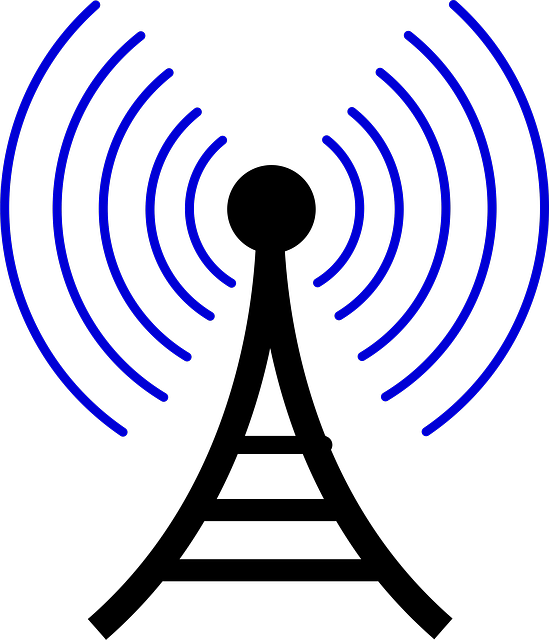
\includegraphics[width=5cm]{images/RapportLogo}\\[0.8cm]
    \textsc{\LARGE Aalborg Universitet}\\[0.6cm]
    \textsc{\Large ITC\\[2mm]3. Semester}\\[0.8cm]

    % Title
    \titlerule \\[0.4cm]
    { \huge \bfseries P2 -- CanSat}\\[0.1cm]
    \titlerule \\
    \raggedleft{\Large{\sffamily A219}} \\[1.4cm]
    % Author and supervisor
    \begin{minipage}[t]{0.49\textwidth}
      \begin{flushleft} \large
        \vspace{0pt} 
        \emph{Forfattere:}\\
        Navn \textsc{efternavn}\\
        Navn \textsc{efternavn}\\
        Navn \textsc{efternavn}\\
        Navn \textsc{efternavn}\\
        Navn \textsc{efternavn}
      \end{flushleft}
    \end{minipage}
    \begin{minipage}[t]{0.49\textwidth}
      \begin{flushright} \large
        \vspace{0pt}
        \emph{Vejledere:} \\
        Vejleder \textsc{efternavn} \\
        Bivejleder \textsc{efternavn}
      \end{flushright}
    \end{minipage}


    \vfill
%    \textit{Denne rapport må ikke gengives uden aftale med forfatterne}\\
    \vspace{1cm}
    % Bottom of the page
    \centering
    {\large December 2012}

\end{titlingpage}

%%% Local Variables: 
%%% mode: latex
%%% TeX-master: "../../master"
%%% End: 

\def\navnA{NAVN}
\def\navnB{NAVN}
\def\navnC{NAVN}
\def\navnD{NAVN}
\def\navnE{NAVN}

\ifx\titlepageleftcolumnwidth\undefined
\newlength{\titlepageleftcolumnwidth}
\newlength{\titlepagerightcolumnwidth}
\fi
\setlength{\titlepageleftcolumnwidth}{0.5\textwidth-\tabcolsep}
\setlength{\titlepagerightcolumnwidth}{\textwidth-2\tabcolsep-\titlepageleftcolumnwidth}
% create title page
\thispagestyle{empty}
\noindent%
\begin{tabular}{@{}ll@{}}
  \parbox{\titlepageleftcolumnwidth}{
    \iflanguage{danish}{%
      
\includegraphics[width=\titlepageleftcolumnwidth]{images/aau_logo_da}
    }{%
      \includegraphics[width=\titlepageleftcolumnwidth]{images/aau_logo_en}
    }
  } &
  \parbox{\titlepagerightcolumnwidth}{\raggedleft\sffamily\small
    % department and address
    % \textbf{Institut for Elektroniske Systemer}\\
    % Fredrik Bajers Vej 7\\
    % DK-9220 Aalborg Ø\\
    % \href{http://es.aau.dk}{http://es.aau.dk}
    \textbf{3. Semester ved Det Teknisk-Naturvidenskabelige og Det Sundhedsvidenskabelige Fakultet}\\
    Strandvejen 12--14\\
    DK-9000 Aalborg\\
    \href{http://tnb.aau.dk}{http://tnb.aau.dk}
  }\medskip\\
  \parbox[t]{\titlepageleftcolumnwidth}{
    \textbf{Titel:}\\ Trådløs Enkoder\medskip\par
    \textbf{Tema:}\\ Computer Engineering\medskip\par
    \textbf{Projektperiode:}\\ Efterårssemestret 2012\medskip\par
    \textbf{Projektgruppe:}\\ 351\medskip\par
    \textbf{Deltager(e):}\\ 
    \navnA\\ 
    \navnB\\
    \navnC\\
    \navnD\\
    \navnE\\
    \navnF\\
    \navnG\medskip\par
    \textbf{Vejledere:}\\ VEJLEDER \\ BIVEJLEDER \medskip\par
    \textbf{Oplagstal:} 1\medskip\par
    \textbf{Sidetal:} \pageref{LastPage}\medskip\par
    \textbf{Afleveringsdato:}\\ 19. december 2012
  } &
  \parbox[t]{\titlepagerightcolumnwidth}{%
    \textbf{Synopsis:}\medskip\par
    \fbox{\parbox{\titlepagerightcolumnwidth-2\fboxsep-2\fboxrule}{%
        SYNOPSIS
%%% Local Variables: 
%%% mode: latex
%%% TeX-master: "../../master"
%%% End: 

      }}
  }\\
\end{tabular}\\

\parbox{\linewidth}{
  \vspace{0.8cm}
  \centering
  \foreach \i in {\navnA,\navnB,\navnC,\navnD,\navnE,\navnF,\navnG}{
    \parbox[t][1.8cm]{4.2cm}{
      \centering
      \hrulefill\\
      \i
    }\hfill
  }
}
\vfill
\noindent{\footnotesize\emph{The content of this report is freely available, but publication (with reference)
    may only be pursued due to agreement with the author.}}

\clearpage
%%% Local Variables: 
%%% mode: latex
%%% TeX-master: "../../master"
%%% End: 

\frontmatter
\chapter*{Forord}
Forord

\section*{Læsevejledning}
\paragraph{Opdeling} TEXT

\paragraph{Bilag} TEXT

\paragraph{Kildeangivelse} TEXT

%%% Local Variables:
%%% mode: latex
%%% TeX-master: "../../master.tex"
%%% End:
\newpage
\tableofcontents
\mainmatter

\chapter{Indledning}
\label{cha:indledning}
I dette afsnit vil der blive beskrevet hvad en enkoder er og hvilke typer enkodere der findes.\\[5mm]

Der er to forskellige slags enkoder-typer. En absolut enkoder og en inkrementel enkoder.\\[5mm]

Den absolutte enkoder gemmer sin position når strømmen fjernes fra systemet og det er muligt at få fat i denne position straks efter strømmen til systemet er etableret. Forholdet mellem den fysiske position og den værdi enkoderen har er noget der bliver lavet når enkoderen samles. En absolut enkoder behøves ikke at have et bestemt reference punkt, som er et fast punkt, som enkoderen bruger til at vide, hvor den befinder sig.\\[5mm] 

En inkrementel enkoder derimod har ikke et fast forhold mellem den fysiske position og enkoderen værdi men kan ændre sig fra den ene gang til den anden. Den inkrementelle enkoder kan have behov for at navigere til referencepunktet for at den nøjagtigt kan registrere positioner.\\[5mm]

Selve opbygningen af disse enkoder-typer kan enten være en mekanisk eller en optisk… når jeg finder ud af forskellen kommer der mere!!!

%%% Local Variables:
%%% mode: latex
%%% TeX-master: "../../master"
%%% End:


\section{Initierende problem}
\label{sec:initierende-problem}
TEXT
\begin{itemize}
\item ITEM1

\item ITEM2

\item ITEM3
\end{itemize}

%%% Local Variables:
%%% mode: latex
%%% TeX-master: "../../master"
%%% End:

\section{Metode og dataindsamling}
\label{sec:metode}

%%% o Lcal Variables:
%%% mode: latex
%%% TeX-master: "../master"
%%% End:



\chapter{Problemanalyse}
\label{cha:problemanalyse}

% Problemformulering
\chapter{Problemformulering}
\label{cha:problemformulering}
Problemformuleringen er defineret således: 
\begin{quote}
  TEXT
\end{quote}
%%% Local Variables: 
%%% mode: latex
%%% TeX-master: "../master"
%%% End: 


% Kravspecifikation
\chapter{Kravspecifikation}
\label{cha:kravspecifikation}
\begin{indledning}

\end{indledning}

% Generel beskrivelse
\section{Generel beskrivelse}
\input{sections/kravspecifikation/generelbeskrivelse}

% Systemanalyse

% Funktionsbeskrivelser


% Brugerprofil
\input{sections/kravspecifikation/brugerprofil}

% Antagelser og Afhængigheder


\section{Specifikke krav}
\label{sec:speckrav}

% Eksterne Grænseflader

% Funktionelle krav


% Ydelses krav


% Design krav


% Software krav
%\input{sections/kravspecifikation/softwareKrav}

\section{Andre Krav}
\label{sec:andre-krav}

% Lovgivnings krav


% Miljø krav


% Økonomiske krav


% Problemafgrænsning


\begin{tail}
TAIL
\end{tail}

\chapter{Testspecifikation}
\label{cha:testspecifikation}
\begin{indledning}
INDLEDNING
\end{indledning}

\begin{tail}
TAIL
\end{tail}


\chapter{Prototype}
\label{cha:prototype}
\begin{indledning}
INDLEDNING
\end{indledning}


\begin{tail}
  TAIL
\end{tail}

\chapter{Implementering}
\label{cha:implementering}

\begin{indledning}
  INDLEDNING
\end{indledning}

\begin{figure}[htbp]
  \centering
  \includegraphics[width=\linewidth]{images/produkt}
  \caption{PRODUKT}
  \label{fig:produkt}
\end{figure}


\chapter{Accepttest}
\label{cha:accepttest}
\begin{indledning}
  indledning til accepttest med udgangspunkt i kravspec
\end{indledning}

%%% Local Variables: 
%%% mode: latex
%%% TeX-master: "../../master"
%%% End: 


\chapter{Konklusion}
\label{cha:konklusion}
\input{sections/opsamling/konklusion}


\chapter{Perspektivering}
\label{cha:perspektivering}
\begin{indledning}
TEXT indledning til perspektivering
\end{indledning}
TEXT
%%% Local Variables: 
%%% mode: latex
%%% TeX-master: "../../master"
%%% End: 


\appendix

%\listoffixmes

% \nocite{*}
% \bibliographystyle{plain}
\bibliographystyle{dk-plain}
\bibliography{bib/kilder}


\end{document}

%%% Local Variables: 
%%% mode: latex
%%% TeX-master: t
%%% End: 
